% !TEX program = xelatex
% Analysis 2 (M2, week 3) report -- generated from docs/report.md by
%     python -m tools.report_to_latex
% Do not edit this file by hand: edit the Markdown and regenerate, or the two will drift apart.
%
% Compile from the docs folder, twice (the second pass resolves the layout):
%     cd docs && xelatex report.tex && xelatex report.tex
% XeLaTeX or LuaLaTeX is required -- the text contains Vietnamese names and the symbols
% ² × § ± Δ → −, which pdfLaTeX with T1 encoding cannot set.
\documentclass[11pt,a4paper]{article}
\usepackage[margin=2.3cm,top=2.5cm,bottom=2.5cm,footskip=1.1cm]{geometry}
\usepackage{fontspec}
\setmainfont{DejaVu Serif}
\setsansfont{DejaVu Sans}
\setmonofont[Scale=0.86]{DejaVu Sans Mono}
\usepackage{booktabs}
\usepackage{array}
\usepackage{adjustbox}
\usepackage{float}
\usepackage{graphicx}
\usepackage{enumitem}
\usepackage{listings}
\usepackage{xcolor}
\usepackage{fancyhdr}
\usepackage{caption}
\usepackage[hidelinks]{hyperref}
\graphicspath{{figures/}}
\captionsetup{font=small,labelfont=bf,skip=4pt}
\setlist[itemize]{leftmargin=1.4em,itemsep=2pt,topsep=3pt,parsep=0pt}
\setlist[enumerate]{leftmargin=1.7em,itemsep=2pt,topsep=3pt,parsep=0pt}
\setlength{\parskip}{4pt}
\setlength{\parindent}{0pt}
\pagestyle{fancy}
\fancyhf{}
\fancyhead[L]{\small Analysis 2 (M2, week 3)}
\fancyhead[R]{\small\thepage}
\renewcommand{\headrulewidth}{0.4pt}
\lstset{basicstyle=\ttfamily\footnotesize,breaklines=true,frame=single,
        framerule=0.3pt,rulecolor=\color{black!40},backgroundcolor=\color{black!3},
        columns=fullflexible,keepspaces=true,showstringspaces=false,
        aboveskip=6pt,belowskip=6pt}
\title{\bfseries Analysis 2 report (M2, week 3)\\[2pt]
       \large used-car valuation and listing screening}
% TODO: put the team names on the line below before submitting.
\author{Week 3 team}
\date{8 November 2026}

\begin{document}
\maketitle
\thispagestyle{empty}
\begin{abstract}
We built a used-car price guide and a screening layer for Vietnamese listings, from \textbf{100,887 ads across eight platforms}, frozen as a snapshot on 31 October 2026. We model \texttt{log1p(price\_vnd)} and split the data by duplicate group instead of by row, so the same car posted on four sites cannot show up on both sides of the split. On validation (14,964 listings) a tuned LightGBM with the full feature set reaches \textbf{R²(log) 0.9471}, with \textbf{MAPE 11.4\%} and a \textbf{median absolute percentage error of 6.2\%}: a typical ad gets a price within about 6\% of what the seller is asking, and the global-median baseline (0.8773) is beaten by seven points. We scored the \textbf{test split exactly once}, after freezing the model and its parameters: \textbf{R²(log) 0.9487, MAPE 10.9\%, median APE 6.1\%}, and the 80\% price band covered \textbf{81.9\%} of asking prices. The same band, plus an Isolation Forest, gives every validation listing one of four labels: \textbf{81.7\% Fair, 8.9\% Bargain, 8.9\% Overpriced, 0.6\% Suspicious}. That last one is 83 ads for a human to read — which is the whole point of the screening layer. Two things matter more than the score. The ceiling here is \textbf{data, not modelling}: nine model families sit inside 0.937–0.947, fifty tuning fits buy +0.0009, and the learning curve is still climbing at 70,000 rows. And the honest headline is not the leaderboard: \texttt{Bargain} does not mean "buy this", the worst errors are deposit-style prices rather than model failures, and any future model change has to be reported as a limitation, because the holdout has been spent. Every number below is what the artefact produced on the frozen splits. Nothing was re-run, re-selected or rounded toward a nicer figure after the test split was opened. There is one number that is optimistic because it was chosen on validation, and §8.2 says which and by how much.
\end{abstract}
\tableofcontents
\newpage


\section*{Headline numbers}
\addcontentsline{toc}{section}{Headline numbers}

\begin{table}[H]
\centering
\footnotesize
\setlength{\tabcolsep}{4pt}
\begin{adjustbox}{max width=\textwidth}
\begin{tabular}{@{}lll@{}}
\toprule
 & Value & Section \\
\midrule
Model shipped & LightGBM, \texttt{full} features, frozen tuned parameters & §5.1 \\
Validation (14,964 listings) & R²(log) \textbf{0.9471} · MAPE \textbf{11.4\%} · median APE \textbf{6.2\%} · MAE \textbf{82.1 million VND} & §5.1 \\
Test (14,980 listings, evaluated once) & R²(log) \textbf{0.9487} · MAPE \textbf{10.9\%} · median APE \textbf{6.1\%} · MAE \textbf{89.7 million VND} & §5.2 \\
80\% price interval on test & covers \textbf{81.9\%} of asking prices & §5.2, §7 \\
Listings flagged on val & \textbf{8.9\%} Bargain · \textbf{8.9\%} Overpriced · \textbf{0.6\%} Suspicious & §7 \\
Canary floor (\texttt{median} 0.8773 → floor 0.946) & beaten by \textbf{+0.0011} R² and \textbf{−0.2} points MAPE — real, and small & §5.1, §8.2 \\
\bottomrule
\end{tabular}
\end{adjustbox}
\end{table}

\begin{table}[H]
\centering
\footnotesize
\setlength{\tabcolsep}{4pt}
\begin{adjustbox}{max width=\textwidth}
\begin{tabular}{@{}lll@{}}
\toprule
Section & Numbers come from & Command that regenerates them \\
\midrule
1 Pipeline & \texttt{split\_summary.json} & \texttt{python -m src.data\_prep.pipeline} \\
2 Data quality & \texttt{missing\_report.json}, \texttt{normalize\_report.json} & \texttt{python -m src.data\_prep.missing} \\
3 EDA & \texttt{docs/eda\_summary.md} + 5 figures & \texttt{python -m tools.eda\_summary} \\
4 Features & \texttt{feature\_ablation.json}, \texttt{cardinality\_study.json}, \texttt{model\_extras.json} & \texttt{python -m src.features.build\_features --ablate} · \texttt{python -m tools.model\_extras} \\
5.1 Benchmark & \texttt{docs/benchmark.md} & \texttt{python -m src.models.benchmark} \\
5.2 Test & \texttt{docs/test\_evaluation.md} & \texttt{python -m src.models.train --split test --at-m2} \\
6 Errors & \texttt{docs/error\_taxonomy.md}, \texttt{docs/case\_studies.md} & \texttt{python -m tools.error\_report} \\
7 Labelling & \texttt{anomaly\_labels.csv}, \texttt{anomaly\_thresholds.json} & \texttt{python -m src.models.anomaly} \\
8 Limitations & — & — \\
9 Conclusions & — & — \\
A Reproduction & — & \texttt{python -m tools.clean\_check} \\
B Artefact inventory & \texttt{data/master/*} & see the table in B \\
C Metric glossary & — & — \\
\bottomrule
\end{tabular}
\end{adjustbox}
\end{table}

\section{Pipeline}

We froze the dataset on 31 October and have not touched it since. \texttt{master\_clean\_dataset.csv} (100,887 rows) goes through \texttt{src.data\_prep.pipeline}, which splits by \texttt{duplicate\_group\_id} (seed 42), then takes the cohort and imputes, then builds \texttt{\{train,val,test\}\_features\_\{minimal,full\}.csv}. The split comes out at \textbf{70.1\% / 14.93\% / 14.97\%} (70,244 / 14,964 / 14,980 rows once features are built). There are \textbf{75,496 duplicate groups} and none of them straddles two splits, so a car cross-posted on four sites cannot sit in both train and val.

Four checks run before a number is allowed into this report:

\begin{table}[H]
\centering
\footnotesize
\setlength{\tabcolsep}{4pt}
\begin{adjustbox}{max width=\textwidth}
\begin{tabular}{@{}lll@{}}
\toprule
Check & Command & Result on this snapshot \\
\midrule
Merged dataset & \texttt{python -m tools.audit\_master} & see the last run log \\
Source contract & \texttt{python -m tools.validate\_source\_csv} & PASS per source \\
Feature leak & \texttt{python -m tools.model\_gate} & PASS — no forbidden column, no copy of the target, all three partitions share one column set, no group straddles a split \\
Unit tests & \texttt{python -m unittest discover -s tests} & 180 tests, OK (2026-11-08) \\
\bottomrule
\end{tabular}
\end{adjustbox}
\end{table}

Every model fits \texttt{log1p(price\_vnd)}, and we report each metric in \textbf{both} log and VND space, so no model gets to show only the flattering number. The test split is scored \textbf{once} — that story is in §5.2.

\section{Data quality}

\begin{itemize}
  \item \textbf{100,887 rows} in the master, \textbf{100,868 with a price}. We drop the 19 without one instead of imputing — you do not invent the thing you are predicting.
  \item \textbf{75,496 duplicate groups} across 100,887 ads, so cross-posting is real. Splitting by group is what stops val and test from being inflated by the same car listed on several sites.
  \item \textbf{Missing rates on train}: \texttt{engine\_capacity} \textbf{61.2\%}, \texttt{sub\_model\_trim} \textbf{55.7\%}, \texttt{seller\_type} \textbf{34.1\%}, \texttt{origin} \textbf{28.6\%}, \texttt{seats} \textbf{21.3\%}, \texttt{body\_type} \textbf{18.6\%}, \texttt{mileage\_km} \textbf{12.7\%}, \texttt{fuel\_type} 0.7\%, \texttt{transmission} 1.5\%. The first two are a real limit on what the model can do, not an implementation detail — \texttt{docs/data\_limitations.md} has the full list.
  \item \textbf{Brand names}: 164 spellings collapse to \textbf{146 brands} (\texttt{Hyundai}/\texttt{HYUNDAI}, \texttt{Mercedes Benz}/\texttt{Mercedes-Benz}, \texttt{VinFast}/\texttt{Vinfast}, \texttt{LandRover}/\texttt{Land Rover}). Skip this and the brand column is noise, with 18 brands split in two.
  \item \textbf{10,906 train rows} carry at least one \texttt{quality\_flags} entry. The model never sees the flag — it is banned as a feature — so those rows are learned like any other. The flag is our judgement about the ad, not a property of the car.
  \item \textbf{Prices on train}: median 520 million, P10 199 million, P90 1.479 billion VND.
  \item \textbf{Volume by source}: bonbanh 21,223 · oto.com.vn 20,764 · chotot 13,631 (19,428 overall) · tinbanxe 5,355 · muaban 4,921 · carpla 2,932 · vucar 1,515 · \textbf{carmudi 366}.
\end{itemize}

\section{What the data looks like (EDA)}

Source: \texttt{data/master/master\_clean\_dataset.csv} — \textbf{100,887 ads} before the price window, \textbf{100,803} after keeping 10 million to 50 billion VND. The 84 dropped rows (0.08\%) are all deposit-style placeholders or typos; the raw maximum was 465 trillion VND. Province names get cleaned before anything is counted (case- and accent-insensitive, plus an alias table), otherwise \texttt{TP HCM} and \texttt{TP.HCM} count as two markets and every regional number is wrong.

\subsection{Five figures, and the number each one has to justify}

\begin{table}[H]
\centering
\footnotesize
\setlength{\tabcolsep}{4pt}
\begin{adjustbox}{max width=\textwidth}
\begin{tabular}{@{}lll@{}}
\toprule
Figure & What it shows & The number to remember \\
\midrule
\texttt{fig1\_price\_distribution.png} & price distribution, drawn on a log10 axis & the raw VND scale has an extreme right tail; log10 nearly symmetrises it, with a residual tail above roughly 10\textasciicircum{}9.5 VND — which is the visual argument for fitting \texttt{log1p(price\_vnd)} \\
\texttt{fig2\_price\_by\_source.png} & median price by platform & 420 million (muaban.net) → 645 million (carpla): \textbf{×1.54} \\
\texttt{fig3\_price\_by\_province.png} & median price by province & TP.HCM 38,271 + Hà Nội 33,079 = \textbf{71\%} of volume; top-12 median spread \textbf{×1.7} \\
\texttt{fig4\_price\_by\_year.png} & median price by model year & 225 million (2010) → 699 million (2025), rising almost monotonically \\
\texttt{fig5\_price\_per\_km\_by\_segment.png} & price per 1,000 km by segment & segments spread \textbf{×9.4} on price per km against \textbf{×3.5} on absolute price \\
\bottomrule
\end{tabular}
\end{adjustbox}
\end{table}

\textbf{Figure 1 — price distribution.} The x-axis is \texttt{log10(asking price, VND)}. On the raw VND scale the tail runs to hundreds of billions and no model would fit it; on the log scale the bulk sits symmetrically around 8.7, with a residual right tail above roughly 10\textasciicircum{}9.5 VND. That is the picture behind the \texttt{log1p} target used in §5.

\begin{figure}[H]
\centering
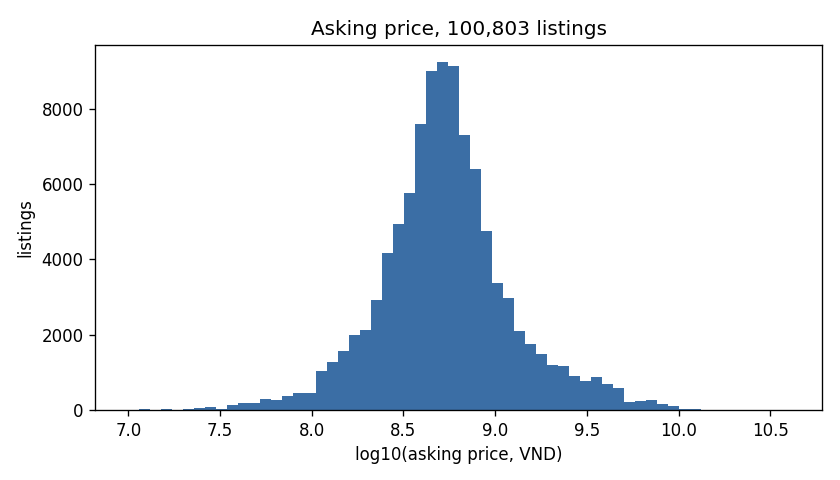
\includegraphics[width=\textwidth]{figures/fig1_price_distribution.png}
\caption{Price distribution}
\end{figure}

\textbf{Figure 2 — median price by platform.} A factor of 1.54 between the cheapest and dearest platform with at least 500 listings.

\begin{figure}[H]
\centering
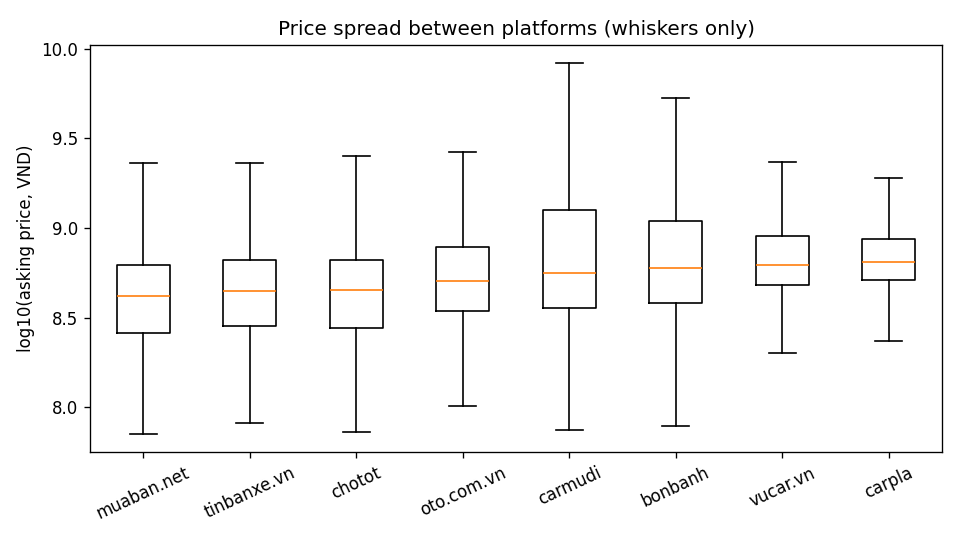
\includegraphics[width=\textwidth]{figures/fig2_price_by_source.png}
\caption{Median price by platform}
\end{figure}

\textbf{Figure 3 — median price by province.} The two largest markets carry 71\% of the volume; the top-12 median spread is 1.7×.

\begin{figure}[H]
\centering
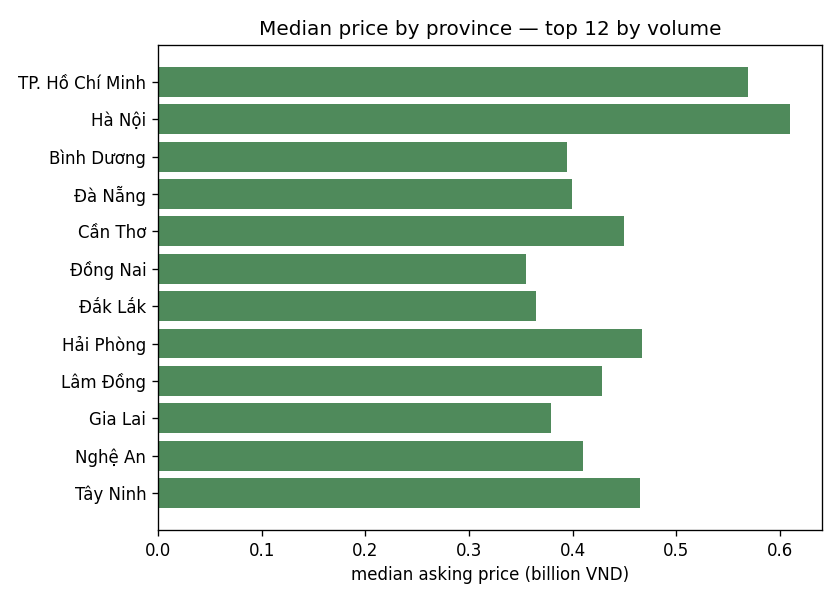
\includegraphics[width=\textwidth]{figures/fig3_price_by_province.png}
\caption{Median price by province}
\end{figure}

\textbf{Figure 4 — median price by model year.} The depreciation curve the model has to learn, 2010–2026.

\begin{figure}[H]
\centering
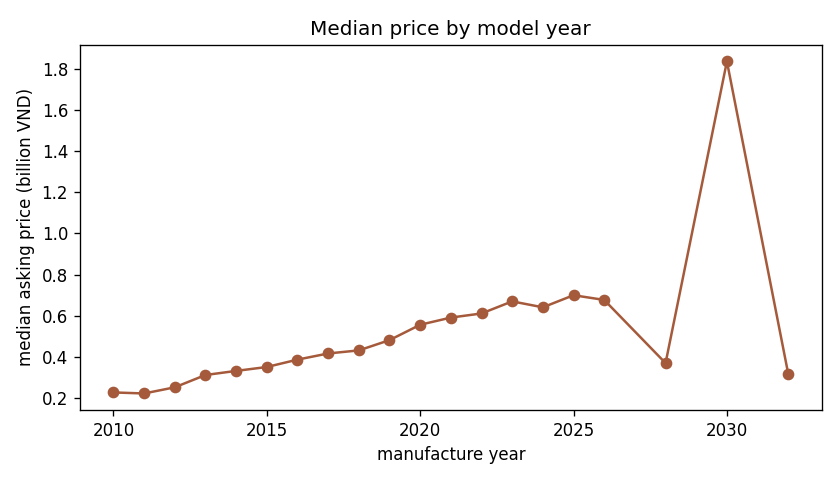
\includegraphics[width=\textwidth]{figures/fig4_price_by_year.png}
\caption{Median price by model year}
\end{figure}

\textbf{Figure 5 — price per 1,000 km by segment.} Segments spread 9.4× on this ratio against 3.5× on absolute price, so mileage does not normalise a segment away.

\begin{figure}[H]
\centering
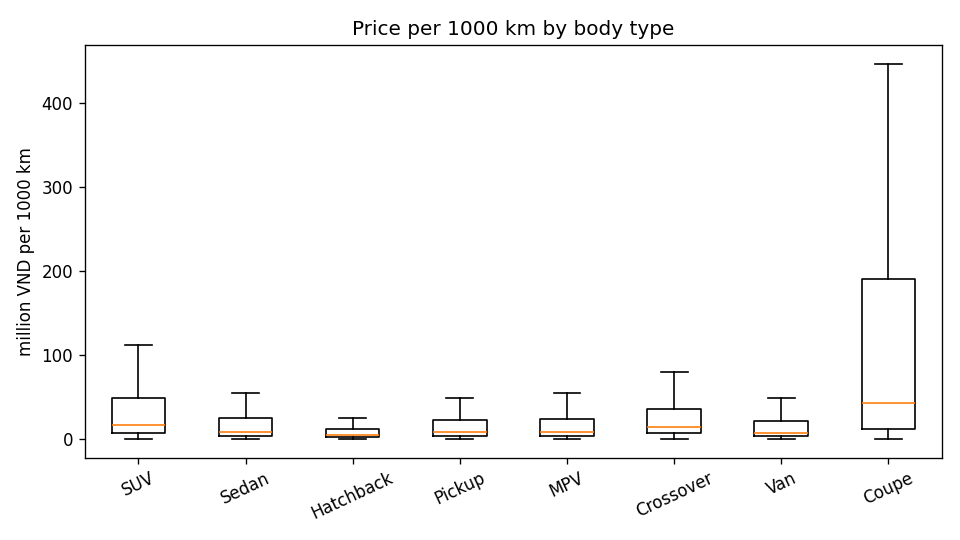
\includegraphics[width=\textwidth]{figures/fig5_price_per_km_by_segment.png}
\caption{Price per 1,000 km by segment}
\end{figure}

\subsection{Three readings that change later sections}

\begin{enumerate}
  \item \textbf{Price per km splits the segments more than absolute price does — and mileage is still weak.} Take the eight segments plotted in Figure 5, every one with at least 900 ads: price per 1,000 km runs from 4.6 million (Hatchback) to 42.7 million (Coupe), \textbf{×9.4}, while absolute price only runs from 265 million to 934 million, \textbf{×3.5}. So mileage does not "normalise" a segment away. For the model itself, §4.2 measures what dropping \texttt{mileage\_km} and \texttt{km\_per\_year} actually costs: \textbf{ΔR² 0.0001}.
  \item \textbf{\texttt{body\_type} is missing on 18.2\% of the window (18.6\% of train)} — a fifth of the market cannot be put in a segment at all, so every "by segment" sentence in this report is about the other 82\%.
  \item \textbf{Small platforms differ in distribution, not just in volume.} carmudi has 546 ads, vucar 2,124, carpla 4,179 — yet carpla's median asking price is 1.54× muaban's. That is why §6 reports error per platform instead of one MAPE, and why §8.1 says carmudi is too small to stand as its own segment.
\end{enumerate}

\subsection{What the model cannot see}

The asking price, not the transaction price; no accident, service, ownership or legal history; four rows carry a model year that cannot be real (1025, 2028, 2030, 2032) and nine have none at all; \texttt{engine\_capacity} is missing on 61.2\% of train, so a large share of cars cannot be told apart by displacement. We carry these into §6 and §8.1 instead of treating them as noise.

\section{Features}

\subsection{Two tables, one whitelist}

\begin{itemize}
  \item \textbf{minimal} — raw columns plus vehicle age: \texttt{manufacture\_year}, \texttt{mileage\_km}, \texttt{engine\_capacity}, \texttt{seats}, \texttt{vehicle\_age}, and the original categoricals.
  \item \textbf{full} — adds \texttt{km\_per\_year}, \texttt{engine\_per\_seat}, \texttt{age\_band}, \texttt{brand\_age\_band}, \texttt{is\_luxury\_segment} (a brand list, \textbf{not} a price rule), \texttt{province\_group}, \texttt{brand\_retention\_rate}, \texttt{province\_price\_index}, \texttt{n\_imputed}.
\end{itemize}

Any statistic used to build a feature (encoders, price indices, retention rates) is fitted on \textbf{train only} and then applied to val/test. \texttt{tools.model\_gate} checks the result afterwards for a leaked or copied target.

\subsection{Group ablation — what each feature group is worth}

We drop one group at a time and refit Ridge on 20,000 rows, as assigned. ΔR² is how much R²(log) falls when the group goes, measured against a \textbf{0.9184} baseline:

\begin{table}[H]
\centering
\footnotesize
\setlength{\tabcolsep}{4pt}
\begin{adjustbox}{max width=\textwidth}
\begin{tabular}{@{}llrl@{}}
\toprule
Group dropped & Columns & R²(log) left & ΔR² \\
\midrule
timing & \texttt{manufacture\_year}, \texttt{vehicle\_age}, \texttt{age\_band}, \texttt{brand\_age\_band} & 0.7904 & \textbf{+0.1280} \\
cat\_identity & \texttt{brand}, \texttt{model}, \texttt{model\_group} & 0.8656 & \textbf{+0.0528} \\
cat\_spec & \texttt{transmission}, \texttt{fuel\_type}, \texttt{origin}, \texttt{body\_type}, \texttt{seller\_type} & 0.9109 & +0.0075 \\
size & \texttt{engine\_capacity}, \texttt{engine\_per\_seat}, \texttt{seats} & 0.9149 & +0.0035 \\
source & \texttt{source\_platform} & 0.9154 & +0.0030 \\
flags & \texttt{n\_imputed}, \texttt{is\_luxury\_segment} & 0.9169 & +0.0015 \\
usage & \texttt{mileage\_km}, \texttt{km\_per\_year} & 0.9183 & +0.0001 \\
geo & \texttt{province\_group}, \texttt{province\_price\_index}, \texttt{brand\_retention\_rate} & 0.9187 & −0.0003 \\
\bottomrule
\end{tabular}
\end{adjustbox}
\end{table}

Two readings, both against what we expected going in, so both go in plainly:

\begin{enumerate}
  \item \textbf{Age and identity are 90\% of the value} (ΔR² 0.1280 + 0.0528). Dropping mileage moves R² by 0.0001 — in this dataset the odometer is simply not a pricing signal, however much it feels like one.
  \item \textbf{The geo group adds nothing} (ΔR² is slightly negative). That backs the decision to keep the two price statistics out of the default preprocessor: dropping them costs nothing and takes away a target leak waiting to happen.
\end{enumerate}

\subsection{Cardinality: categorical beats target encoding here}

From \texttt{docs/cardinality\_research.md} (LightGBM on 20,000 rows, only the brand/model encoding changes): \texttt{brand}+\texttt{model} as categorical \textbf{0.9319} · \texttt{model\_group} \textbf{0.9313} · \texttt{model} \textbf{0.9304} · out-of-fold target encoding \textbf{0.9178}. At this cardinality — 1,912 models, 103–146 brands — target encoding \textbf{does not win}. It is a variance-control trick for linear models, not an accuracy gain, and we say so rather than dressing it up as a technique that paid off.

\subsection{What the fitted model actually uses}

From \texttt{tools.model\_extras} (its own LightGBM run: R²(log) 0.9458, MAPE 11.6\% on val):

\begin{table}[H]
\centering
\footnotesize
\setlength{\tabcolsep}{4pt}
\begin{adjustbox}{max width=\textwidth}
\begin{tabular}{@{}lrr@{}}
\toprule
Feature & Permutation importance (RMSE, log space) & sd \\
\midrule
\texttt{brand\_age\_band} & 0.5096 & 0.0812 \\
\texttt{manufacture\_year} & 0.2621 & 0.0362 \\
\texttt{model} & 0.2314 & 0.0392 \\
\texttt{model\_group} & 0.1803 & 0.0353 \\
\texttt{brand} & 0.1317 & 0.0210 \\
\texttt{engine\_capacity} & 0.1301 & 0.0244 \\
\bottomrule
\end{tabular}
\end{adjustbox}
\end{table}

The top four are all "what car, which year" — the same story the ablation tells from the other side. Partial dependence agrees: hold \texttt{manufacture\_year} at 2011 and the model predicts 493 million, at 2021 it says 793 million, at 2025 it says 858 million.

\textbf{Seed stability} (3 seeds, 20,000 rows, 300 trees): 0.9305 / 0.9312 / 0.9308 → mean \textbf{0.9308 ± 0.0003}. That ±0.0003 is exactly why §5.1 uses a paired test instead of a bare ranking: anything below about 0.001 is the noise you get from re-running the same code.

\textbf{Learning curve} (7,024 / 17,561 / 35,122 / 70,244 train rows): 0.8947 → 0.9107 → 0.9311 → 0.9440. It is still climbing at the last point, which means the ceiling here is \textbf{data and features}, not model capacity — the strongest argument we have against spending another day on hyperparameters.

\section{Models}

\subsection{Benchmark on val (14,964 rows)}

Nine model families, two feature sets. Three combinations got tuned within a \textbf{600 s budget — 25 draws × 2 grouped folds = 50 fits} — and everything else runs on fixed parameters; the \texttt{tuning} column of \texttt{docs/benchmark.md} marks which is which. Every number on this page is \textbf{val}; the test split only shows up in §5.2.

\begin{table}[H]
\centering
\footnotesize
\setlength{\tabcolsep}{4pt}
\begin{adjustbox}{max width=\textwidth}
\begin{tabular}{@{}llrrrrrrrrl@{}}
\toprule
Features & Model & R²(log) & RMSE(log) & R²(VND) & MAE (VND) & MAPE & MAPE clean & median APE & s & tuning \\
\midrule
full & \textbf{lightgbm+tuned} & \textbf{0.9471} & 0.1904 & 0.9215 & 82,087,205 & 11.4\% & 10.3\% & 6.2\% & 468.5 & 25×2 \\
full & catboost & 0.9465 & 0.1914 & 0.9134 & 91,143,312 & 12.0\% & 10.9\% & 6.9\% & 447.8 & fixed \\
minimal & lightgbm+tuned & 0.9464 & 0.1916 & 0.9162 & 84,155,488 & 11.6\% & 10.4\% & 6.3\% & 138.8 & 25×2 \\
full & lightgbm & 0.9462 & 0.1919 & 0.9213 & 82,441,420 & 11.5\% & 10.4\% & 6.3\% & 16.7 & fixed \\
minimal & lightgbm & 0.9447 & 0.1945 & 0.9151 & 84,885,802 & 11.7\% & 10.6\% & 6.4\% & 5.4 & fixed \\
full & \textbf{xgboost+tuned} & 0.9440 & 0.1957 & 0.9010 & \textbf{78,041,635} & \textbf{11.0\%} & \textbf{9.8\%} & 5.9\% & 326.7 & 25×2 \\
minimal & catboost & 0.9438 & 0.1961 & 0.9056 & 95,474,212 & 12.3\% & 11.2\% & 7.1\% & 264.8 & fixed \\
minimal & xgboost+tuned & 0.9413 & 0.2004 & 0.8983 & 80,995,302 & 11.3\% & 10.1\% & 6.2\% & 269.4 & 25×2 \\
full & rf & 0.9411 & 0.2008 & 0.9094 & 87,698,367 & 12.1\% & 10.7\% & 6.4\% & 149.8 & fixed \\
full & xgboost & 0.9409 & 0.2011 & 0.8952 & 78,256,273 & 11.1\% & 9.8\% & \textbf{5.7\%} & 22.3 & fixed \\
minimal & catboost+tuned & 0.9395 & 0.2035 & 0.8962 & 100,674,556 & 13.0\% & — & 7.5\% & 308.7 & 1×2 \\
minimal & xgboost & 0.9388 & 0.2046 & 0.8914 & 80,850,994 & 11.3\% & 10.1\% & 6.0\% & 11.2 & fixed \\
minimal & rf & 0.9370 & 0.2076 & 0.8960 & 94,182,039 & 12.6\% & 11.2\% & 6.7\% & 120.8 & fixed \\
full & ridge & 0.8970 & 0.2655 & 0.8200 & 141,897,201 & 18.0\% & 16.4\% & 10.4\% & 6.1 & fixed \\
full & median (baseline) & 0.8773 & 0.2899 & 0.8703 & 101,649,813 & 18.8\% & 13.2\% & 7.3\% & 1.8 & fixed \\
minimal & ridge & 0.8746 & 0.2930 & 0.7824 & 157,731,450 & 20.6\% & 18.6\% & 11.5\% & 4.5 & fixed \\
full & elasticnet & 0.8722 & 0.2958 & 0.7458 & 174,713,377 & 21.2\% & 19.3\% & 13.4\% & 90.5 & fixed \\
full & lasso & 0.8561 & 0.3139 & 0.7136 & 190,664,684 & 22.9\% & 20.9\% & 14.8\% & 37.4 & fixed \\
full & knn & 0.8553 & 0.3147 & 0.7387 & 181,201,164 & 22.8\% & 20.8\% & 13.4\% & 1.5 & fixed \\
minimal & elasticnet & 0.8507 & 0.3198 & 0.7138 & 192,621,090 & 23.7\% & 21.5\% & 14.7\% & 17.4 & fixed \\
minimal & knn & 0.8372 & 0.3338 & 0.7273 & 194,474,953 & 25.9\% & 23.5\% & 14.8\% & 1.1 & fixed \\
minimal & lasso & 0.8344 & 0.3367 & 0.6868 & 207,337,967 & 25.5\% & 23.1\% & 16.2\% & 19.4 & fixed \\
\bottomrule
\end{tabular}
\end{adjustbox}
\end{table}

\texttt{MAPE clean} throws out rows whose asking price is below a quarter of the estimate — the deposit-style ads §6 is about. One row, \texttt{minimal}/\texttt{catboost+tuned}, shows \texttt{—}: its search stopped after a single draw inside the 600 s budget, and the run was written before this column existed. The row stays as it is rather than spending another 300 s to fill one cell of a search that never finished. The two \texttt{median} rows are identical because the baseline ignores the feature set completely: a "model" that only knows the global median already sits at R²(log) 0.8773.

\textbf{We fixed the primary metric before reading the table: R²(log)} — the thing the models actually minimise, and the thing the canary floor is stated in. That order matters, because the metric picks the winner:

\begin{enumerate}
  \item \textbf{The canary floor is 0.946 R²(log) / 11.6\% MAPE; the best row is 0.9471 / 11.4\%.} It clears both, by +0.0011 and −0.2 points. Nothing here is a step change from complexity: untuned LightGBM lands on 0.9447–0.9462, i.e. \emph{right on} the floor, so "the complexity is worth it" rests on the tuned row alone.
  \item \textbf{Tuning buys almost nothing: +0.0009 R²} (0.9462 → 0.9471), for 50 fits and 16.7 s → 468.5 s. A paired Wilcoxon on absolute percentage error says the gap is real (p = 7.8e-05) against a seed sd of 0.0003 — real, and still irrelevant to anyone using the thing.
  \item \textbf{CatBoost and LightGBM tie} (0.9465 vs 0.9462 untuned). Wilcoxon prefers catboost (p = 2.3e-15), but the R² gap is 0.0003 — exactly one seed sd — and catboost is \emph{worse} on MAPE (12.0\% vs 11.5\%).
  \item \textbf{XGBoost wins in VND space and loses on ranks.} \texttt{xgboost+tuned} has the best MAE (78.0 million), MAPE (11.0\%), clean MAPE (9.8\%) and median APE (5.9\%), yet the paired Wilcoxon against \texttt{lightgbm+tuned} calls it \textbf{worse} (p = 5.8e-12). Both are true: it wins on expensive cars and loses by small margins on the many cheap ones. This is the whole reason for naming the primary metric up front instead of afterwards.
  \item \textbf{The median baseline beats ridge on median APE} (7.3\% vs 10.4\%) while scoring lower on R² (0.8773 vs 0.8970). A model that looks better by R² can be worse in the middle of the distribution — the kind of wrong call the median-APE column exists to catch.
\end{enumerate}

\texttt{full} beats \texttt{minimal} by about 0.0015 R² on the untuned pair (0.9462 vs 0.9447). Small, real (Wilcoxon p = 7.4e-07) against a 0.0003 noise floor — worth keeping, not worth calling a big improvement.

\textbf{What we ship in \texttt{predictions\_\{val,test\}.csv}: lightgbm+tuned / full}, with the parameters frozen as \texttt{n\_estimators=900, learning\_rate=0.03, num\_leaves=63, min\_child\_samples=20}. Running it back through \texttt{--params} gives exactly \textbf{0.9471 / 0.1904 / 82,087,205 / 11.4\%} in 31.9 s instead of 468.5 s, so the artefact reproduces without repeating the search. We took LightGBM over catboost for two reasons: better MAPE (11.4\% vs 12.0\%), and it emits quantiles directly, so the P10/P90 band in §7 does not need a third model.

\subsection{Test — the single evaluation}

We scored the test split \textbf{once}, after the model and its parameters were frozen. The record is \texttt{docs/test\_evaluation.md}; the interval check is \texttt{docs/intervals\_test.md}.

\begin{table}[H]
\centering
\footnotesize
\setlength{\tabcolsep}{4pt}
\begin{adjustbox}{max width=\textwidth}
\begin{tabular}{@{}lrr@{}}
\toprule
Metric & val (14,964) & \textbf{test (14,980)} \\
\midrule
R²(log) & 0.9471 & \textbf{0.9487} \\
RMSE(log) & 0.1904 & 0.1869 \\
R²(VND) & 0.9215 & 0.9026 \\
MAE (VND) & 82,087,205 & 89,731,484 \\
MAPE & 11.4\% & \textbf{10.9\%} \\
MAPE clean & 10.3\% & 10.1\% \\
median APE & 6.2\% & 6.1\% \\
band coverage (nominal 80\%) & 81.70\% & \textbf{81.91\%} \\
\bottomrule
\end{tabular}
\end{adjustbox}
\end{table}

Three things come out of that table:

\begin{enumerate}
  \item \textbf{The test split is not suspiciously easy.} R²(log) and MAPE come out 0.0016 / 0.5 points \emph{better} than val — the kind of gap you get between two splits of the same distribution, not evidence that the holdout was kind to us.
  \item \textbf{MAE and R²(VND) go the other way} (89.7 vs 82.1 million; 0.9026 vs 0.9215), because they are absolute VND numbers and the test mix has more expensive cars. Same model, opposite readings — the lesson from §5.1, now on held-out data.
  \item \textbf{The band survives the move} — 81.91\% against a nominal 80\%, split as 8.62\% below P10 and 9.47\% above P90. Calibrating on train OOF did not quietly fit the band to val.
\end{enumerate}

What we \textbf{will not} do now: re-tune, re-pick a model, widen the band, or score the test split again. The split is spent, and \texttt{docs/test\_evaluation.md} refuses a second write unless \texttt{--force} is passed by hand. Anything we change from here goes in as a limitation (§8.2), never as a fresh test number.

\section{Error analysis}

\begin{itemize}
  \item \textbf{Median APE 6.2\%, MAPE 11.4\%} on val (test: 6.1\% / 10.9\%). Two different measurements, both correct: MAPE gets dragged by the right tail, median APE describes an ordinary ad.
  \item \textbf{By bucket} (\texttt{docs/error\_taxonomy.md}, with the rules in \texttt{tools/error\_report.py::bucket}, so every count can be re-derived): under 200 million — \textbf{1,461} rows, median APE \textbf{13.2\%}, mean Δ \textbf{+24.7\%}. The model \textbf{over}-prices cheap cars, because that bucket is where the deposit and bait prices live. Extreme odometer — \textbf{118} rows, \textbf{9.6\%}. Everything else — \textbf{13,385} rows, \textbf{5.8\%}.
  \item \textbf{By platform}: carmudi \textbf{10.0\%} (105 rows) · chotot 7.1\% (2,874) · muaban 6.7\% (1,044) · tinbanxe 6.5\% (1,124) · carpla 6.3\% (610) · oto.com.vn 5.9\% (4,369) · bonbanh 5.9\% (4,529) · vucar 4.8\% (309). Error is not spread evenly, and the smallest platform has the worst number — one MAPE for the whole market would hide exactly that.
  \item \textbf{By price decile}: the cheapest decile (< 200 million) sits at median APE \textbf{13.0\%}, roughly double the deciles above it (6.8\% / 5.4\%). The model is weakest where the buyer has the least money.
  \item \textbf{The 25 worst rows} (\texttt{docs/error\_audit\_25.md}, read by hand): \textbf{24 of 25 are deposit-style prices}, 6 have placeholder odometers, 1 is a genuine duplicate. That tail is a \textbf{data} problem, not a modelling one — no amount of tuning fixes an ad that posts 7\% of a car's value to farm phone numbers.
  \item \textbf{Three case studies} (\texttt{docs/case\_studies.md}, picked by rule so they reproduce): \texttt{MUA\_71248118}, a 2022 Toyota Corolla Cross asking \textbf{7.35 billion} against a \textbf{631 million} estimate (Δ −91.4\%); \texttt{CHOTOT\_134989809}, a 2024 Aion Y Plus with \textbf{999,998 km} (Δ +488\%); \texttt{CARPLA\_F8W47}, a 2024 Audi Q5 import asking \textbf{218 million} against \textbf{2.06 billion} (Δ +843\%).
  \item \textbf{Feature importance} (\texttt{data/master/feature\_importance.csv}): \texttt{brand\_age\_band} 0.510 · \texttt{manufacture\_year} 0.262 · \texttt{model} 0.231 · \texttt{model\_group} 0.180 · \texttt{brand} 0.132 · \texttt{engine\_capacity} 0.130. The first three are "what car, which year" again, matching §4.2.
\end{itemize}

None of those three failure modes is a model bug. They are a deposit price, an edited odometer, and an import advertised at a domestic-looking price. §8.2 draws the conclusion: this product needs \emph{data} — transaction prices, service history — more than it needs another model.

\section{Labelling suspicious and mispriced listings}

How it works (\texttt{src/models/anomaly.py}, thresholds in \texttt{data/master/anomaly\_thresholds.json}):

\begin{enumerate}
  \item \textbf{Band} — P10/P90 from LightGBM's quantile triple, calibrated on \textbf{train OOF} (never on val or test). It covers \textbf{81.70\%} of val prices and \textbf{81.91\%} of test prices against a nominal 80\%.
  \item \textbf{Isolation Forest} — 300 trees, \texttt{max\_samples} 4096, on the val feature matrix (numbers as they are, categoricals as codes). Its job is to find "outside the band \textbf{and} odd in feature space".
  \item \textbf{Review threshold} — the 97th percentile of the forest score, i.e. \textbf{3.00\%} of val rows (449 ads) land in the review queue. That is a \textbf{budget for how many ads a human will read}, not an estimate of how many bad ads exist.
\end{enumerate}

Labels are produced on \textbf{val} (14,964 ads). We deliberately leave the test split unlabelled — it is only there for §5.2.

\begin{table}[H]
\centering
\footnotesize
\setlength{\tabcolsep}{4pt}
\begin{adjustbox}{max width=\textwidth}
\begin{tabular}{@{}lrrl@{}}
\toprule
Label & Ads & Share & Median Δ (asking vs estimate) \\
\midrule
Fair & 12,225 & 81.7\% & −0.6\% \\
Bargain & 1,331 & 8.9\% & \textbf{+19.7\%} \\
Overpriced & 1,325 & 8.9\% & \textbf{−14.7\%} \\
Suspicious & 83 & 0.6\% & +8.9\% \\
\bottomrule
\end{tabular}
\end{adjustbox}
\end{table}

Of the 449 ads above the forest threshold, only \textbf{83} are also outside the band. So \texttt{Suspicious} is much narrower than "the review queue", and 83 is the number to give a moderator.

\textbf{By price band} — the labels pile up at the cheap end, which ties back to §6:

\begin{table}[H]
\centering
\footnotesize
\setlength{\tabcolsep}{4pt}
\begin{adjustbox}{max width=\textwidth}
\begin{tabular}{@{}lrrrrr@{}}
\toprule
Price band & Ads & Bargain & Overpriced & Suspicious & \% flagged \\
\midrule
< 200 million & 1,501 & 336 & 49 & \textbf{25} & \textbf{27.3\%} \\
200–400 million & 3,555 & 374 & 232 & 17 & 17.5\% \\
400–700 million & 5,170 & 370 & 409 & 12 & 15.3\% \\
700 million – 1.5 billion & 3,226 & 211 & 386 & 15 & 19.0\% \\
> 1.5 billion & 1,512 & 40 & 249 & 14 & 20.0\% \\
\bottomrule
\end{tabular}
\end{adjustbox}
\end{table}

\textbf{By platform} — most Bargains on tinbanxe.vn (9.9\%), most Overpriced on carpla (12.6\%):

\begin{table}[H]
\centering
\footnotesize
\setlength{\tabcolsep}{4pt}
\begin{adjustbox}{max width=\textwidth}
\begin{tabular}{@{}lrrr@{}}
\toprule
Platform & Ads & \% Bargain & \% Overpriced \\
\midrule
bonbanh & 4,529 & 9.5\% & 9.3\% \\
oto.com.vn & 4,369 & 8.3\% & 9.8\% \\
chotot & 2,874 & 8.9\% & 7.3\% \\
tinbanxe.vn & 1,124 & \textbf{9.9\%} & 6.6\% \\
muaban.net & 1,044 & 9.5\% & 7.7\% \\
carpla & 610 & 8.5\% & \textbf{12.6\%} \\
vucar.vn & 309 & 3.9\% & 10.7\% \\
carmudi & 105 & 5.7\% & 3.8\% \\
\bottomrule
\end{tabular}
\end{adjustbox}
\end{table}

Three things worth saying out loud:

\begin{enumerate}
  \item \textbf{\texttt{Bargain} does not mean "buy this".} 336 of the 1,331 Bargains are under 200 million — the exact bucket §6 calls deposit and bait prices (24 of the 25 worst rows). The label says "below the model". The model cannot tell a deposit from a car.
  \item \textbf{Labels move with the band, so they move with the model.} Swap the model or recalibrate the band and the shares change. That is why §6 quotes the coverage, and why the forest threshold is written into \texttt{anomaly\_thresholds.json} — so a later run can be compared instead of trusted.
  \item \textbf{The 3\% review rate is a choice about workload.} Set it to 2\% or 5\% and you change how many ads a person reads, not the nature of the problem. 83 Suspicious ads out of 14,964 is few enough to read by hand, and that is the whole deliverable.
\end{enumerate}

\section{Limitations}

\subsection{Data}

\begin{itemize}
  \item \textbf{Asking price, not transaction price.} Everything here means "the model matches the asking price". We do not know the haggling margin or what was actually paid, so error measured on asking prices is an \textbf{upper bound} on error against real sale prices — and this snapshot cannot tell us how loose that bound is.
  \item \textbf{Fields we need and do not have}: \texttt{engine\_capacity} 61.2\% missing, \texttt{sub\_model\_trim} 55.7\%, \texttt{body\_type} 18.2\% of the window, \texttt{mileage\_km} 12.7\%. No accident, service, ownership or legal-history data at all.
  \item \textbf{One snapshot, no time.} We exclude the listing date because it leaks, which also means the model knows nothing about seasonality or how prices drift month to month.
  \item \textbf{Uneven sources}: carmudi has 546 ads in total and 105 in val, too few to be a segment. Anything we say per platform about carmudi or vucar rests on a small sample.
  \item \textbf{19 rows without a price are dropped}, not imputed. \textbf{4 rows with impossible model years} (1025, 2028, 2030, 2032) stay in the feature table and are treated as categorical values rather than hand-edited.
\end{itemize}

\subsection{Model and process}

\begin{itemize}
  \item \textbf{The ceiling is data, not modelling.} Nine families land inside 0.937–0.947, 50 tuning fits buy 0.0009, and the learning curve is still climbing (0.8947 → 0.9440 from 7k to 70k rows). Real mileage, a proper brand/model taxonomy, seasonality — any of those is worth more than another model.
  \item \textbf{The ranking depends on the metric.} LightGBM+tuned wins R²(log) at 0.9471; XGBoost+tuned wins MAE, MAPE and median APE while the paired Wilcoxon calls it worse. We fix R²(log) as primary because it is the training objective and the metric the canary floor is written in — and we say plainly that a different primary metric would give a different winner.
  \item \textbf{The tuned score is a bit optimistic.} 0.9471 is the best of 25 draws picked on the same 14,964 val rows, so it should sag on new data. It actually went \emph{up} to 0.9487 on test, but that is one measurement, not proof against the optimism.
  \item \textbf{The band does not always contain the point forecast} — 1.80\% of val rows and 1.78\% of test rows. The band comes from quantile models, the point comes from the mean model, so nothing forces one inside the other. It is recorded in \texttt{docs/intervals.md}; forcing the band to swallow the point would widen it and wreck the calibration.
  \item \textbf{The test split is spent.} \texttt{docs/test\_evaluation.md} is written once and the tool refuses to overwrite it. Anything we change from here goes in as a limitation, with no second test run — otherwise the "evaluated once" line in this report stops meaning anything.
\end{itemize}

\section{Conclusions and next steps}

\subsection{What we know now}

\begin{enumerate}
  \item \textbf{The model is good enough for price guidance, and we have a real holdout to say so.} R²(log) 0.9487 and median APE 6.1\% on 14,980 ads nobody touched during development. A typical ad gets within about 6\% of its asking price. This is not a demo that happens to fit val.
  \item \textbf{The gap to the baseline is the number worth quoting, not the gap to the ceiling.} The global-median baseline scores 0.8773; the shipped model scores 0.9471 on val. Seven points of R² is what "predict price from which car and which year" actually buys. The last 0.05 is what this dataset cannot give us.
  \item \textbf{The complexity pays for itself, but barely.} Against the canary floor of 0.946 the shipped model wins by 0.0011. Enough to keep it, not enough to celebrate — §5.1 says the same thing in the same words, which is why the rest of that table is worth trusting.
  \item \textbf{The intervals are calibrated and they travel.} 81.70\% coverage on val, 81.91\% on test, against a nominal 80\%, with the calibration fitted on train out-of-fold rows only. This is the piece that would break first if the feature set changed.
  \item \textbf{The screening layer produces a workload, not a verdict.} 83 Suspicious ads out of 14,964 is a queue a person clears in a morning. The part to distrust is the label, not the count.
\end{enumerate}

\subsection{What the product should promise, and what it should not}

What the evidence supports: \textbf{"a starting number for a negotiation, plus a short review queue."} What it does not support: \textbf{contract-grade valuation}. The reason is structural — every label here is an \emph{asking} price and the haggling margin is not in the data. As a limitation that is honest; as a feature claim it is a promise the data cannot keep.

In practice: quote the interval, not the point. Quote \texttt{median APE 6.1\%} for a typical ad, and say out loud that the cheapest decile is twice as bad (13.0\%). Put a warning next to \texttt{Bargain} that a price below P10 is more often a deposit than a deal — 24 of the 25 worst rows in §6 are exactly that.

\subsection{What we would do next, in order}

\begin{table}[H]
\centering
\footnotesize
\setlength{\tabcolsep}{4pt}
\begin{adjustbox}{max width=\textwidth}
\begin{tabular}{@{}rll@{}}
\toprule
Priority & Work & Why it comes first \\
\midrule
1 & \textbf{Transaction prices} (sold listings, dealer invoices) & turns an asking-price model into a valuation model; nothing else changes the target definition \\
2 & \textbf{Real odometer history} (service records, registration data) & \texttt{mileage\_km} is 12.7\% missing and worth ΔR² 0.0001 as it stands; the \emph{true} value is the signal the model currently lacks \\
3 & \textbf{Model-year × variant taxonomy} (\texttt{sub\_model\_trim} is 55.7\% missing) & the top three features are all "what car, which year"; filling the missing half is the cheapest real gain \\
4 & \textbf{Time axis} (listing date as seasonality, not as a leak) & with a second snapshot, month-of-year becomes learnable; with one, it is not \\
5 & More tuning, more model families & measured at +0.0009 for 50 fits; this is the last thing worth doing, not the first \\
\bottomrule
\end{tabular}
\end{adjustbox}
\end{table}

\subsection{What must not happen}

Any of items 1–5 changes the data or the model, which means a \textbf{new snapshot and a re-opened freeze}. The current test number (0.9487) then becomes history: it stays in this report as the measurement of \emph{this} model on \emph{this} split, and a new number comes from a new one-shot evaluation — never from re-scoring the same split until it looks better. Two guards keep that honest after submission: \texttt{docs/test\_evaluation.md} is written once and refuses to be overwritten, and \texttt{python -m src.models.train --split test} exits unless \texttt{--at-m2} is passed.

\appendix
\section{Reproduction runbook}

The data snapshot is not in the repo (\texttt{data/master/*} is git-ignored — \texttt{docs/data\_handover.md} §5 explains why). A fresh clone plus the mandatory download reproduces every number in this report:

\begin{lstlisting}
# 0. environment
pip install -r requirements.txt          # Python 3.12; lightgbm >= 4.5, pandas >= 3.0

# 1. snapshot: put these three files in data/master/
#    train_cohort_imputed.csv, val_cohort_imputed.csv, test_cohort_imputed.csv
#    (01_week3_mandatory/ on Drive; verify with SHA256SUMS.txt)

# 2. features
python -m src.features.build_features --features full --split all

# 3. the shipped model on val, with the parameters frozen before the test run
python -m src.models.train --model lgbm --features full --quantiles --label lightgbm+tuned \
  --params '{"n_estimators":900,"learning_rate":0.03,"num_leaves":63,"min_child_samples":20}'
#   -> R²(log) 0.9471, MAE 82,087,205, MAPE 11.4%, band coverage 81.7%

# 4. the one-shot test evaluation (writes docs/test_evaluation.md once)
python -m src.models.train --model lgbm --features full --quantiles --split test --at-m2 \
  --label lightgbm+tuned \
  --params '{"n_estimators":900,"learning_rate":0.03,"num_leaves":63,"min_child_samples":20}'
#   -> R²(log) 0.9487, MAPE 10.9%, band coverage 81.91%

# 5. downstream artefacts
python -m src.models.anomaly --predictions data/master/predictions_val.csv   # §7
python -m tools.error_report                                                # §6
python -m tools.check_intervals                                             # §5.2, §7
python -m tools.model_gate                                                  # leak gate
\end{lstlisting}

Two shortcuts. \texttt{python -m tools.clean\_check} pulls \texttt{HEAD} into a temp folder and runs features → train → gate → tests there, which is how "the committed tree is enough" gets \emph{checked} instead of assumed. And \texttt{python -m src.models.benchmark} rebuilds the §5.1 table, though it is slow: three models × 600 s of tuning. Timings on the machine that produced this report: features about 20 s, train about 45 s including quantiles, gate and tests about 10 s.

\section{Artefact inventory}

Everything a reviewer needs to check a number, and nothing that has to be taken on trust:

\begin{table}[H]
\centering
\footnotesize
\setlength{\tabcolsep}{4pt}
\begin{adjustbox}{max width=\textwidth}
\begin{tabular}{@{}lll@{}}
\toprule
Artefact & Contents & Used by \\
\midrule
\texttt{data/master/predictions\_val.csv} & 14,964 × 15: ids, vehicle, asking price, \texttt{y\_pred\_*}, \texttt{p10\_vnd}, \texttt{p90\_vnd}, residual, APE & §5.1, §6, §7 \\
\texttt{data/master/predictions\_test.csv} & 14,980 × 15, same contract, written once at M2 & §5.2 \\
\texttt{data/master/model\_results.json} & append-only ledger, one row per (model, features, seed, holdout, frozen) & §5.1, §5.2 \\
\texttt{docs/model\_results.json} & committed copy of the ledger, so the numbers travel with the repo & §5.1, §5.2 \\
\texttt{docs/benchmark.md} & the §5.1 table with tuning budget and per-row timings & §5.1 \\
\texttt{docs/test\_evaluation.md} & the single test evaluation, written once, refuses overwrite & §5.2 \\
\texttt{docs/intervals.md}, \texttt{docs/intervals\_test.md} & band coverage by platform, on val and on test & §5.2, §7 \\
\texttt{data/master/anomaly\_labels.csv} & per-listing label, band, forest score, reason & §7 \\
\texttt{data/master/anomaly\_thresholds.json} & calibrated forest threshold, review rate, label counts & §7 \\
\texttt{docs/error\_taxonomy.md}, \texttt{docs/error\_audit\_25.md} & error buckets, platform/decile breakdowns, the hand-read tail & §6 \\
\texttt{docs/case\_studies.md} & three listings picked by rule, with URLs & §6 \\
\texttt{data/master/feature\_ablation.json}, \texttt{docs/features\_ablation.md} & drop-one-group ΔR² & §4.2 \\
\texttt{data/master/cardinality\_study.json}, \texttt{docs/cardinality\_research.md} & encoding comparison & §4.3 \\
\texttt{docs/model\_extras.md} & permutation importance, partial dependence, seed stability, learning curve & §4.4 \\
\texttt{docs/eda\_summary.md}, \texttt{docs/figures/fig1..fig5} & the EDA tables and the five figures & §3 \\
\texttt{docs/data\_limitations.md}, \texttt{docs/features.md}, \texttt{docs/feature\_formulas.md} & data caveats and the feature definitions & §2, §4, §8 \\
\bottomrule
\end{tabular}
\end{adjustbox}
\end{table}

\section{Metric glossary}

\begin{table}[H]
\centering
\footnotesize
\setlength{\tabcolsep}{4pt}
\begin{adjustbox}{max width=\textwidth}
\begin{tabular}{@{}lll@{}}
\toprule
Term & Definition & Why it is reported \\
\midrule
\textbf{R²(log)} & coefficient of determination on \texttt{log1p(price\_vnd)} — the space the models are trained in & primary metric: it is the training objective and the metric the canary floor is expressed in \\
\textbf{RMSE(log)} & root mean squared error in log space & same space as R²(log), in price-error units \\
\textbf{R²(VND)} & R² on raw VND & shows how much of the \emph{money} variance is explained; always flattering because the distribution is skewed \\
\textbf{MAE (VND)} & mean absolute error in VND & the number a business reader feels; scales with car price \\
\textbf{MAPE} & mean absolute percentage error over all rows & comparable across price levels, but dominated by cheap rows \\
\textbf{MAPE clean} & MAPE after dropping rows whose asking price is below a quarter of the estimate & the same measure without the deposit-price tail (\texttt{docs/error\_audit\_25.md}) \\
\textbf{median APE} & median absolute percentage error & the typical listing rather than the average; immune to the tail \\
\textbf{band coverage} & share of asking prices inside \texttt{[p10\_vnd, p90\_vnd]} & calibration check against the nominal 80\%; a band that does not cover 80\% makes the §7 labels fire at the wrong rate \\
\textbf{canary floor} & R²(log) 0.946 / MAPE 11.6\% from \texttt{tools/baseline\_smoke} & the number any added complexity has to beat to be worth its cost \\
\bottomrule
\end{tabular}
\end{adjustbox}
\end{table}

\end{document}
